% Author: Dr. Matthias Jung, DL9MJ
% Year: 2020
% 
\documentclass[convert = false, border=5pt, varwidth]{standalone}
\usepackage{fontspec}
\setmainfont{Roboto}
\usepackage[siunitx, straightvoltages]{circuitikzgit}
\usepackage{tikz}


\usepackage{tikz,pgfplots}
\usetikzlibrary{arrows}

\usepackage{amsmath}
\usepackage{unicode-math}
\setmathfont{Fira Math}
\setmathfont[range=up]{Roboto}
\setmathfont[range=it]{Roboto-Italic}
\setmathfont[range=\int]{Fira Math}
\usepackage[euler]{textgreek}

\begin{document}

TODO: Bild darüber...

\pgfplotsset{
  every axis plot/.append style={line width=0.8pt},
}
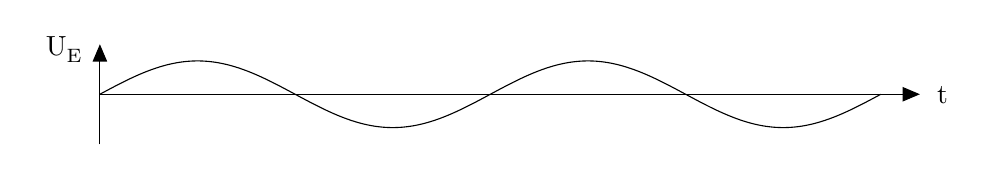
\begin{tikzpicture}
    \draw (10.7, 0.625) node[]{t};
    \draw (-0.45, 1.20) node[]{$\mathrm{U}_\mathrm{E}$};
    \draw (-0.8, 1.20) node[]{~};
    \begin{axis}[%
        /pgf/number format/1000 sep={ },
        /pgf/number format/use comma,        
        axis lines=middle,
        axis line style={-triangle 45},
        width=4.1in,
        height=0.5in,
        scale only axis,
        ytick={0},
        every major tick/.append style={thick, black},
        grid=major,
        grid style={line width=.1pt, draw=gray!10},
        major grid style={line width=.2pt,draw=gray!50},
        xticklabel=\empty,
        yticklabel=\empty,
        xtick style={draw=none},
        ytick style={draw=none},
        xmin=0,
        xmax=4.2*pi,
        ymin=-0.75,
        ymax=0.75,
        xmajorgrids=false,
        ymajorgrids=false,
        tick label style={font=\footnotesize}
    ]
        \addplot[samples=500,domain=0:4.0*pi,smooth,black] {0.5*sin(deg(x))+0}; 
\end{axis}
\end{tikzpicture}%

\end{document}


